\section{Design patterns}

\subsection{UML}
\begin{figure}[h]
\caption{UML arrows}
\centering
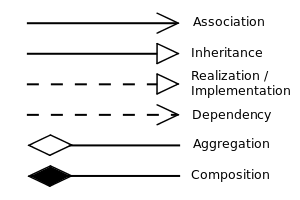
\includegraphics[width=0.5\textwidth]{images/umlArrows.png}
\end{figure}


\begin{figure}[h]
\caption{UML classes}
\centering
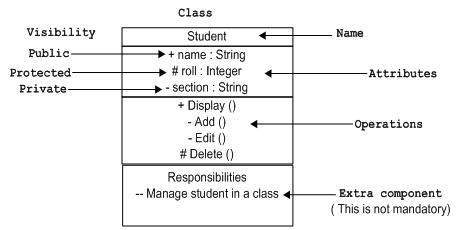
\includegraphics[width=0.5\textwidth]{images/umlClass.jpg}
\end{figure}

\subsection{Dependencies versus microservices}

Dependencies can be included right in your sourcode. Microservices on the other hand are not included at all, but called remotely from your programm. 


\begin{table}[h]
\centering
\caption{Dependencies versus microservices}
\begin{tabular}{@{}lllll@{}}
\toprule
        & Dependencies                                             & Microservices                                                      &  &  \\ \midrule
Changes & You can include the exact needed version of a dependency & Your program needs to adapt immediately if the service API changes &  &  \\
        &                                                          &                                                                    &  &  \\
        &                                                          &                                                                    &  &  \\ \bottomrule
\end{tabular}
\end{table}




\subsection{State pattern}
\begin{figure}[h]
\caption{State design pattern}
\centering
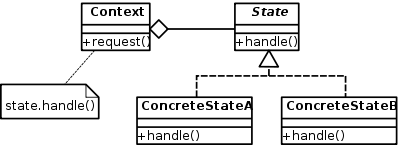
\includegraphics[width=0.5\textwidth]{images/stateDesignPattern.png}
\end{figure}

\subsection{Workflow pattern}

